\section{Models}
\label{sec:models}

\begin{center}
``All models are wrong; some models are useful." (George E.\ P.\ Box)
\end{center}

In the real world, we will, in all likelihood, have to work with data. ``Data-driven decisions" is a common phrase heard today. One thing that can be said is that real world data is messy and complex. Countless factors influence every phenomenon. Some factors are designed and some are purely random. Sometimes a data set is incomplete, missing pieces of data. Yet we may have to work with that data set as if it was complete. Sometimes we are tasked with {\bf forecasting}, which is predicting future data points, given the ones that we have.

\subsection{What is a Mathematical Model?}
\label{ssec:models}
In many different areas, we need tools to simplify a set of data and work with that simplified version of the data. These simplifications must be based on reasonable assumptions that connect to the larger context of the data. Simplifications serve two purposes. First, it may be impossible to take every variable into account. Second, models must often be communicated to others and a simple model is generally more clear and therefore much easier to communicate. This is the essence of what is called {\bf mathematical modeling}\index{Mathematical modeling}, or simply {\bf modeling}\index{Modeling}.

\begin{definition}
A {\bf model} \index{model} or a {\bf mathematical model} is a mathematical framework to help describe some phenomenon, specifically how an input or quantity affects or relates to some output.  A model has three main components:
\begin{enumerate}
    \item One or more input variables, with specific descriptions of what these variables represent, including units.
    \item One or more functions, with specific descriptions of what the output of the functions represent, including units.
    \item A domain and/or range over which the function(s) make sense to use.
\end{enumerate}
Additionally, we may want to consider the following when creating a model.
\begin{itemize}
    \item Identify underlying assumptions that were used to simplify the situation.
    \item Perform a sensitivity analysis to determine if the model is relatively unchanged if the data varies slightly.
\end{itemize}
\end{definition}

For example, one could construct a model to speculate how the price of an item affects the demand for that item, and from that, predict revenue from sales of that item.

It is crucial to state that a model is used to simplify reality and does not dictate or reflect past, present, or future reality with absolute precision. Although good models can be useful for forecasting, decision-making, and filling in missing data. That is the essence of the quote at the beginning of the section by the late George Box, a famous British statistician.

%\begin{wrapfigure}{R}{0.3\textwidth}
\begin{floatingfigure}{0.3\textwidth}
    \centering
    %\vspace{-20pt}
    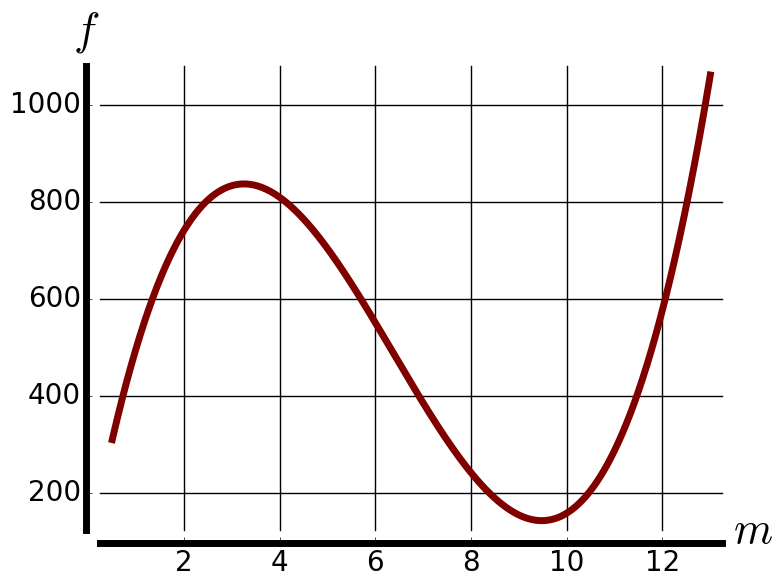
\includegraphics[width=0.3\textwidth]{img/chap1/sec1-3/fig1-3-oil.png}\\
    \caption{Fuel Oil Usage by Plant W in 2016.}
    \label{fig:1-3-oil-curve}
    %\vspace{-12pt}
\end{floatingfigure}
%\end{wrapfigure}

The following is an example of a mathematical model, based on an actual data set from ``Plant W." We will analyze this scenario in several places in this text and.

{\bf Model:} Plant W heats an external tank and powers their operations by burning fuel oil. The rate at which they burned this oil in 2016 can be described by the following model. Let $m$ be the month of the year, with 1 referring to January 1, and 12 referring to December 1, so that $1\le m < 13$. Let $f(m)$ describe the rate at which the fuel burns, in gallons per month. A model for $f(m)$ is
$$f(m) = 5.76m^3 - 109.98m^2 + 532.58m + 70.17\mbox{ gallons per month.}$$
Figure \ref{fig:1-3-oil-curve} plots this curve over the given domain.
%\end{example}
\begin{remark} Note that in this example, we clearly described the input variable, what it represented, a domain that it makes sense over, and gave the units (months). We clearly described the function (the output), what it modeled, and gave the units.
\end{remark}

Examining the graph of the function, we can see that the model makes sense, based on the context. If Plant W is heating a large external tank, then in the winter and early spring, we expect more oil to be used to heat it. This tank may also have retained some heat, as fluids tend to do, from the late summer and fall. We expect a significant drop in oil usage through the late spring and summer months and finally a significant increase in oil usage during the fall and early winter.

Is the model precise? Of course not. First, we know that in 2016 (a leap year), there were months with 29, 30, or 31 days, yet we treated each month as equal. Perhaps a better model would have modeled fuel usage per day. For the sake of clarity, however, we aggregated the days into months; we know immediately that month 6 is June, but do not immediately know which month is day 276, for example.

A second reason that we know that the model is not accurate is that we can't be certain that on January 1, 2016 that Plant W burned oil at a rate of $f(1) = 498.53$ gallons per month. In other words, on January 1, 2016, did Plant W burn $f(1)/31 = 16.08$ gallons of fuel oil? We can be almost certain that they did not, but the actual amount may have been somewhat close to that. Other factors that we didn't consider were the range of temperatures that day and the percentage of the tank that was full. Considering these factors would make the model more accurate, but more complex.

A third item to consider is that in this case, we are dealing with a yearly cycle. We should expect $f(1)$ to be really close to $f(13)$, since both input values would refer to January 1 in 2016 and 2017, respectively. However, we have
$$ f(1) = 498.53 \quad \mbox{and} \quad f(13) = 1061.81 \enspace ,$$
which is a significant difference. Perhaps a better model would attempt to get these two points either closer to each other or make them exactly equal to each other. Section \ref{sec:trig} will describe how to work with periodic or seasonal data such as this. \hfill$\blacksquare$

\subsection{Scatter Plots: Plotting Data in a Spreadsheet}
\label{ssec:plot-data}
Throughout this book, we will use a spreadsheet to plot and analyze data. In the spirit of using free and open-source resources, our examples will use the well-known office suite {\em LibreOffice}\index{LibreOffice}, specifically its spreadsheet software {\em Calc}. LibreOffice is compatible with other office suites and the various menus and wizards are very similar to that of other office suites. {\em LibreOffice} is installed by default in most distributions of the Linux operating system, but the most current version is available for free at {\tt https://www.libreoffice.org/} for Linux and other major operating systems.

In this section, we will see how to create two different kinds of {\bf scatter plots}\index{Scatter plot} in {\em Calc}. A scatter plot is simply a representation of data in which each element of a data set can be represented as a point on a set of coordinate axes. A scatter plot helps to visualize the relationship between variables in a data set.

The first kind of scatter plot is ideal for {\bf time series}\index{Time series}, a data set that is in chronological order and there is at most one data point for every unit of time. Examples include economic data, such as a country's gross domestic product (GDP) over time; financial data, such as the price of a stock or commodity; biological data, such as the population of a species in a region over time; business data, such as a company's sales over time; and so on. Such plots help to identify trends and the strength of that trend.

The following spreadsheet shows the oil usage data of Plant W in 2016.

\begin{table}[ht!]
  \centering
  \resizebox{\textwidth}{!}{%
    \textsf{
    \begin{tabular}{|a*{13}{|c}|}
    \hline
    \rowcolor{shGray} & A & B & C & D & E & F & G & H & I & J & K & L & M\\
    \hline
    1 & \textbf{Month} & Jan. & Feb. & Mar. & Apr. & May & June & July & Aug. & Sep. & Oct. & Nov. & Dec. \\
    \hline
    2 & \textbf{Oil (Gal.)} & 573.0 & 850.0 &  425.3 & 800.1  & 818.9 &  880.9 &  296.5 & 198.7 & 105.4 & 72.0 &  & 638.0\\
    \hline
  \end{tabular}}}
  %\caption{Fuel Oil Usage at Plant W in 2016}
  \label{sh:1-3-oil}
\end{table}

\noindent To make a scatter plot of this data:
  \begin{itemize}
      \item Highlight the data (including the labels).
      \item Select {\tt Insert} from the {\tt LibreOffice Calc} menu.
      \item Select {\tt Chart ...} to bring up the {\bf Chart Wizard}.
      \item Select {\tt Line} and the {\bf Points Only} plot.
      %\item Select {\tt XY (Scatter)} and the {\bf Points Only} plot.
    \end{itemize}
\begin{center}
  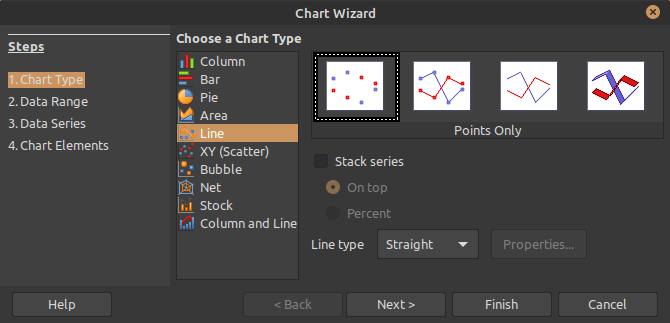
\includegraphics[width = 0.6\textwidth]{img/chap1/sec1-3/line-scatter1.png}
\end{center}
  \begin{itemize}
      \item Click on {\tt Next >}. If you've already highlighted the data, then the wizard should have the correct range.
      \item Select {\tt Data series in rows} and check {\tt First column as label} since the first column are the axis labels of the data.
    \end{itemize}
  \begin{center}
  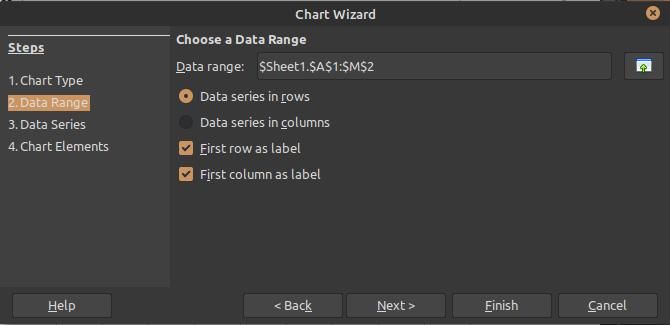
\includegraphics[width = 0.6\textwidth]{img/chap1/sec1-3/scatterplot2.png}
  \end{center}
    \begin{itemize}
      \item Select {\tt 4.\ Chart Elements} on the left panel of the wizard.
      \item Put in appropriate titles and axis labels for the plot.
      \item Other options in this part of the wizard will make the chart more readable.
      \item Select {\tt Finish}.
    \end{itemize}
    \begin{center}
    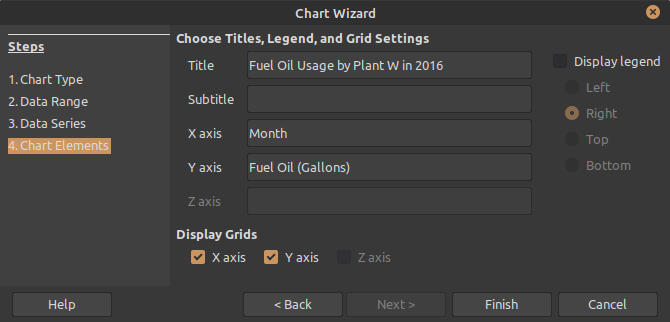
\includegraphics[width = 0.6\textwidth]{img/chap1/sec1-3/scatterplot3-oil.png}
    \end{center}
    \begin{itemize}
      \item Once the wizard is complete, we can make other changes to the chart.
      \item Double-clicking on the plotted points allows you to change the color and shape of the plotted points.
      \item Double-click on the $y$-axis and select the {\tt Scale} tab. Changing the {\tt Major interval} to 200 makes the axis a little more readable.
    \end{itemize}
    \begin{center}
    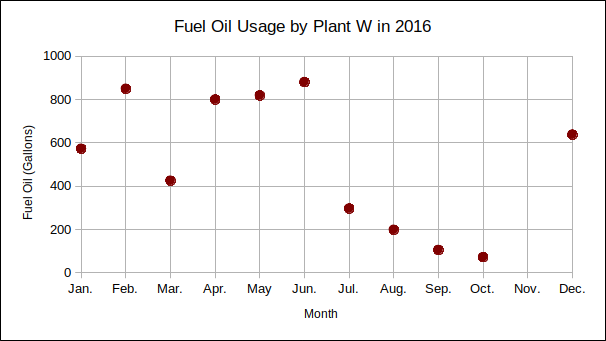
\includegraphics[width = 0.6\textwidth]{img/chap1/sec1-3/scatterplot4-oil.png}
    \end{center}

The second type of scatter plot is more general and seeks to understand the relationship between two variables in a particular phenomenon.

Suppose that you are a new realator in King County, Washington. You want to understand the housing market in the county in order to advise potential home buyers and sellers on reasonable prices for homes. You acquire a data set giving information on 21,613 home sales in King County, WA between May 2, 2014 and May 27, 2015. The following spreadsheet is a very small portion of this data set. To get started, you want to understand the relationship between living space area and the sale price of a home, though there are certainly more variables to consider. It makes more sense to think of the sale price as a function of the living space area, so the $x$-axis will be living space area in square feet and the sale price (in U.S. dollars) will be along the $y$-axis.

\begin{table}[ht!]
  \centering
    \textsf{
    \begin{tabular}{|a*{13}{|c}|}
    \hline
    \rowcolor{shGray} & A & B \\
    \hline
    1 & \textbf{Price (\$)} & \textbf{Living Area (ft$^2$)}  \\
    \hline
    2 & 313000 & 1340 \\
    \hline
    3 & 2384000 & 3650 \\
    \hline
    4 & 342000 & 1930 \\
    \hline
    $\dots$ & $\dots$ & $\dots$\\
    \hline
    21613 & 445500 & 1390\\
    \hline
    21614 & 1310000 & 3750 \\
    \hline
  \end{tabular}}
  \caption{King County Home Sales from May 2, 2014 to May 27, 2015}
  \label{sh:1-3-houses}
\end{table}

\noindent To make a scatter plot of this data:
  \begin{itemize}
      \item Highlight the data (including the labels).
      \item Select {\tt Insert} from the {\tt LibreOffice Calc} menu.
      \item Select {\tt Chart ...} to bring up the {\bf Chart Wizard}.
      \item Select {\tt XY (Scatter)} and the {\bf Points Only} plot.
    \end{itemize}
\begin{center}
  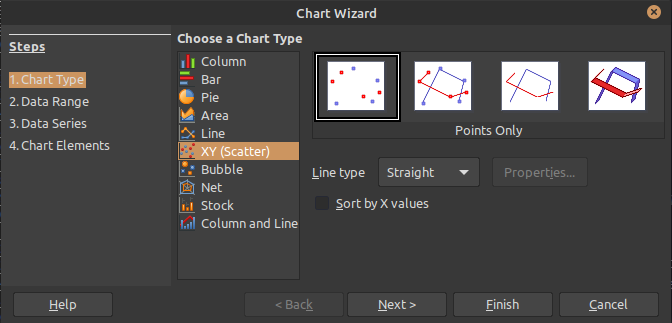
\includegraphics[width = 0.6\textwidth]{img/chap1/sec1-3/scatterplot1.png}
\end{center}
  \begin{itemize}
      \item Click on {\tt Next >}. If you've already highlighted the data, then the wizard should have the correct range.
      \item Select {\tt Data series in columns} and check {\tt First row as label} since the first row are the axis labels of the data.
    \end{itemize}
  \begin{center}
  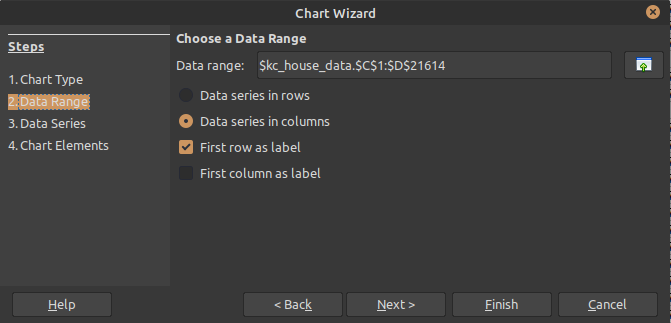
\includegraphics[width = 0.6\textwidth]{img/chap1/sec1-3/scatterplot-column-2.png}
  \end{center}
  \begin{itemize}
    \item Click on {\tt Next >}.
    \item Notice that the $x$-axis data is in Column B and the $y$-axis data is in Column A. In this {\tt Data Series} window, manually adjust this.
    \item In the {\tt Data ranges:} area, click on {\tt X-Values} and {\tt Y-Values} and change the {\tt Range for X-Values} and {\tt Range for Y-Values}, respectively.
  \end{itemize}
  \begin{center}
  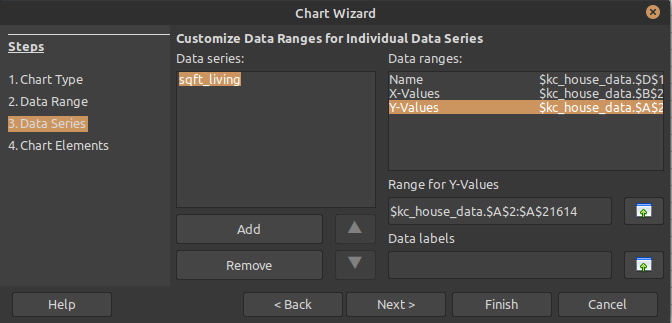
\includegraphics[width = 0.6\textwidth]{img/chap1/sec1-3/scatterplot-column-3.png}
  \end{center}
    \begin{itemize}
      \item Click on {\tt Next >} to go to {\tt 4.\ Chart Elements}.
      \item Put in appropriate titles and axis labels for the plot.
      \item Other options in this part of the wizard will make the chart more readable.
      \item Select {\tt Finish}.
      \item We will adjust the chart as we did above to make it more readable.
    \end{itemize}
    \begin{center}
    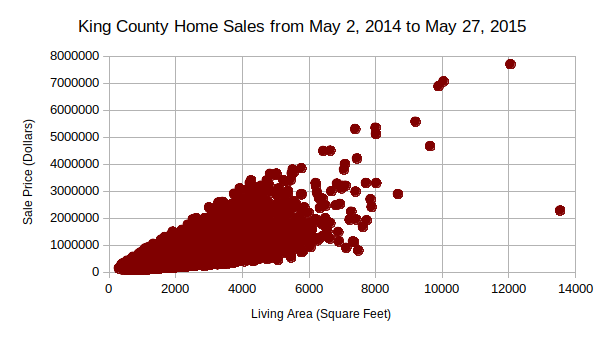
\includegraphics[width = 0.6\textwidth]{img/chap1/sec1-3/fig1-3-houseprices.png}
    \end{center}

We immediately notice a number of things. First, with such a large data set, it is apparent that data is messy. There appears to be a predictable trend but for any living area, there is a very wide price range. Most people looking to buy or sell a house will also not be interested in the data of the very expensive houses, so the data on the large and expensive houses could be ignored. Also, King County covers a large area: Seattle, many of its suburbs, and areas within the Cascade Range. Houses in the city and upscale areas of the suburbs will sell for much more than a similarly sized house in the mountains. For this reason, data and models need to be considered in context.

Now suppose that you are helping a family with three children find a house in Issaquah. The father is a software engineer and the mother homeschools the children and based on their budget, they would consider a house no more than \$400,000. Would you show them this chart? Of course not. We will sort the data and consider homes in Issaquah (ZIP codes 98027, 98029, and 98075) that have sold for \$400,000 or less. However, to attempt to establish a more accurate trend, we will plot data on house prices up to \$600,000.
  \begin{itemize}
    \item Highlight the spreadsheet by clicking on the empty box next to the {\tt A} column designation.
    \item Click on {\tt Data} in the menu.
    \item Select {\tt Sort...}
    \item On the {\tt Options} tab, select {\tt Range contains column labels}.
    \item Go back to {\tt Sort Criteria}. Under {\tt Sort Key 1}, select the ZIP code and {\tt Ascending}.
    \item Under {\tt Sort Key 2}, select the price and {\tt ascending}.
  \end{itemize}
  Gathering this data into a separate spreadsheet, we now have 464 entries. The family wants at least three bedrooms and at least two bathrooms. This narrows our data set to 345 entries, which is more readable.
  \begin{center}
  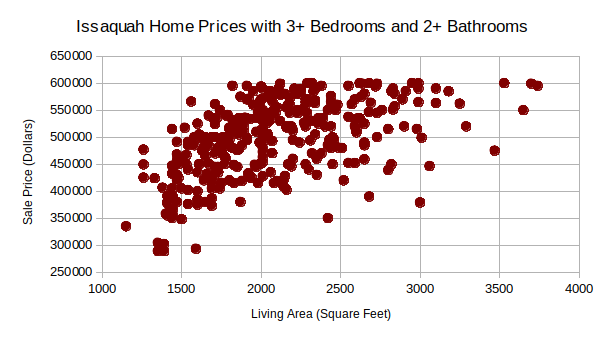
\includegraphics[width = 0.6\textwidth]{img/chap1/sec1-3/issaquah-homes.png}
  \end{center}
  Given this level of context, you, as the real estate agent, and the family have a more accurate picture of the relationship between living area and home price. This would better equip you to make a reasonable offer on a house that comes up for sale.

  The data is still quite messy. It's called a scatter plot for a reason! Though we have elimined much of the data by drilling down and focusing on certain values for some variables, there are more variables to consider. Throughout the book, we will explore various ways to model this data with a curve.
\subsection{Curve Fitting, Interpolation, and Extrapolation}
\label{ssec:cfie}

\begin{wrapfigure}{R}{0.3\textwidth}
%\begin{floatingfigure}{0.3\textwidth}
    \centering
    %\vspace{-20pt}
    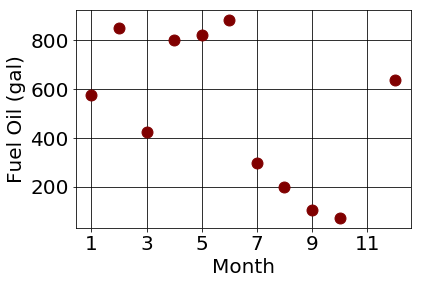
\includegraphics[width=0.3\textwidth]{img/chap1/sec1-3/ex1-3-oil.png}\\
    \caption{Fuel Oil Usage by Plant W in 2016.}
    \label{fig:1-3-oil}
    %\vspace{-20pt}
%\end{floatingfigure}
\end{wrapfigure}
A common and simple way to create a mathematical model from a scatter plot of a data set is to determine a function that is a reasonable fit to the curve, given the scenario. Figure \ref{fig:1-3-oil} gives an example of a scatter plot of data from Table \ref{tab:1-3-oil} that will be used in Example \ref{ex:interpolation}. {\bf Curve fitting}\index{Curve fitting} is a technique in which one creates a continuous function to smooth out discrete data. The curve will generally not ``connect the dots" of a scatter plot of the data, but will give the general behavior of the data. The most common and well-known means to fit a curve to data is by creating a {\bf regression curve}\index{Curve!regression}\index{Regression} of the data. The mathematical details of how to make these curves is outside the scope of this text. It is sufficient to understand that regression curves are {\bf curves of best fit}\index{Curve!best fit} or {\bf best fit curves}.

With an appropriate curve fit to data, we can {\bf interpolate}\index{Interpolation} and {\bf extrapolate}\index{Extrapolation} the data.

\begin{definition}
Using the graph of a function to estimate values between known data points (i.e., within the domain) is called {\bf interpolation}. Making predictions beyond the domain of known data is called {\bf extrapolation}. When a model no longer applies after some point, and extrapolation is unreasonable it is sometimes called \textbf{model breakdown}\index{Model breakdown}.
\end{definition}

\paragraph{Interpolation.} In cases in which there is missing data, we can use interpolation techniques to make educated guesses for the actual data. This is just one example in which interpolation is used. The following example uses regression curves and another simpler technique.

\begin{example}
\label{ex:interpolation}
Plant W, mentioned earlier, powers their operations by burning fuel oil. Table \ref{tab:1-3-oil} below shows how much oil they burned in 2016, but they are missing data from November. (Figure \ref{fig:1-3-oil} gave a scatter plot of this data.) What are some reasonable values for the amount of fuel oil that they burned in November 2016?

\begin{table}[h!]
\centering
\begin{tabular}{l*{12}{c}}
\toprule
Month & Jan. & Feb. & Mar. & Apr. & May & June & July & Aug. & Sep. & Oct. & Nov. & Dec. \\
\midrule
Oil (gal) & 573.0 & 850.0 &  425.3 & 800.1  & 818.9 &  880.9 &  296.5 & 198.7 & 105.4 & 72.0 & ?? & 638.0\\
\bottomrule
\end{tabular}
\caption{Fuel Oil Usage at Plant W in 2016}
\label{tab:1-3-oil}
\end{table}
\begin{solution} We will show two ways to estimate the missing data point. The first is straightforward. The other will use a model developed from a regression curve, applying concepts and techniques that we will learn more about in Section \ref{sec:polynomial}.

A simple way to interpolate a missing data point is to find the average (or mean) of the data point before and the data point after the missing point. With this approach, we have an estimate for the November 2016 fuel oil consumption of
$$\frac{72.0 + 638.0}{2} \mbox{ gallons} = \frac{710.0}{2} \mbox{ gallons} = 355 \mbox{ gallons.}$$

The second method creates a model by finding a curve the best fits the data in Table \ref{tab:1-3-oil}. The volume of fuel oil burned by Plant W in month $m$ of 2016 is
$$f(m) = 5.76m^3 - 109.98m^2 + 532.58m + 70.17\mbox{ gallons.}$$
This model is plotted with the data in Figure \ref{fig:1-3-oil-model}, showing that the model is reasonable.
%\begin{wrapfigure}{R}{0.3\textwidth}
%\begin{floatingfigure}{0.3\textwidth}
\begin{figure}[!ht]
    \centering
    %\vspace{-20pt}
    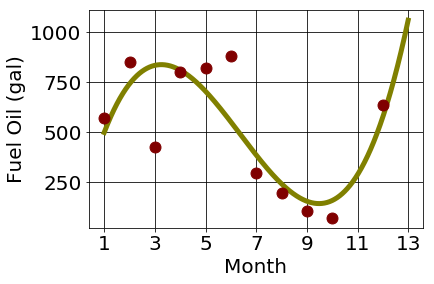
\includegraphics[width=0.6\textwidth]{img/chap1/sec1-3/fig1-3-oil-curve.png}\\
    \caption{Fuel Oil Usage by Plant W in 2016.}
    \label{fig:1-3-oil-model}
    %\vspace{-20pt}
  \end{figure}
%\end{floatingfigure}
%\end{wrapfigure}

From this model, we can estimate that Plant W burned
$$f(11) = 5.76\cdot 11^3 - 109.98\cdot 11^2 + 532.58\cdot 11 + 70.17\mbox{ gallons} = 287.53 \mbox{ gallons}$$
in November (month $m=11$).
\end{solution}\end{example}

\paragraph{Extrapolation.} In contrast to interpolation, extrapolation is more difficult because it involves predicting data points beyond the domain of the data using the trends that currently exist. Extra care must be used to create and justify assumptions used to develop the model that is used to extrapolate.

Let's discuss the following table and plot of winning Men's and Women's 100 meter dash times in the Olympics. As of this writing, the next summer Olympics will be in 2020, so we can extrapolate from the given data to predict the winning times in the next Olympics. When we plot the data, however, many more questions will naturally arise and the answers to those questions will vary depending on the model that we use to describe the data.

\begin{table}[h!]
\centering
\begin{tabular}{l*{11}{r}}
\toprule
Year        & 1928 & 1932 & 1936 & 1948 & 1952 & 1956 & 1960 & 1964 & 1968 & 1972  & 1976 \\
\midrule
Time (M, s) & 10.8 & 10.3 & 10.3 & 10.3 & 10.4 & 10.5 & 10.2 & 10.0 & 9.95 & 10.14 & 10.06 \\
\midrule
Time (W, s) & 12.2 & 11.9 & 11.5 & 11.9 & 11.5 & 11.5 & 11.0 & 11.4 & 11.0 & 11.07 & 11.08 \\
\bottomrule
Year        &  1980 & 1984 & 1988 & 1992 & 1996 & 2000 & 2004 & 2008 & 2012 & 2016 & 2020 \\
\midrule
Time (M, s) & 10.25 & 9.99 & 9.92 & 9.96 & 9.84 & 9.87 & 9.85 & 9.69 & 9.63 & 9.81 & ???? \\
\midrule
Time (W, s) & 11.06 & 10.97 & 10.54 & 10.82 & 10.94 & 11.12 & 10.93 & 10.78 & 10.75 & 10.71 & ???? \\
\bottomrule
\end{tabular}
\caption{Winning Men's and Women's 100 Meter Dash Times in the Olympics}
\label{tab:1-3-dash}
\end{table}

%\begin{wrapfigure}{R}{0.4\textwidth}
%\begin{floatingfigure}{0.4\textwidth}
\begin{figure}[ht!]
    \centering
    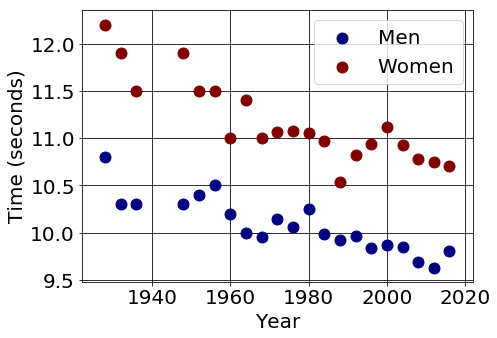
\includegraphics[width=0.4\textwidth]{img/chap1/sec1-3/fig1-3-dash.png}\\
    \caption{Winning Olympic 100-Meter Dash Times}
    \label{fig:1-3-dash}
%\end{wrapfigure}
%\end{floatingfigure}
\end{figure}
Figure \ref{fig:1-3-dash} gives a scatter plot of the data. It's clear that there has been a downward trend in the gold medal times over the past century, but it's not a smooth trend. The data is choppy. The simplest curve-fitting model to smooth out the data is to use a best fit line. In the next section, we will learn how to find best fit lines, but for now, we will describe the model and discuss the model.

{\bf Model: } Let $y$ be the year and $1928\le y\le 2016$. Then the winning men's and women's 100-meter dash times in the Olympics in year $y$ can be described by $m(y)$ and $w(y)$, respectively.
\begin{align}
\label{eq:1-3-dash}
m(y) &= -0.009498y + 28.841\mbox{ seconds}\\
w(y) &= -0.014185y + 39.188 \mbox{ seconds}\nonumber
\end{align}

\begin{floatingfigure}{0.4\textwidth}
%\begin{figure}[ht!]
    \centering
    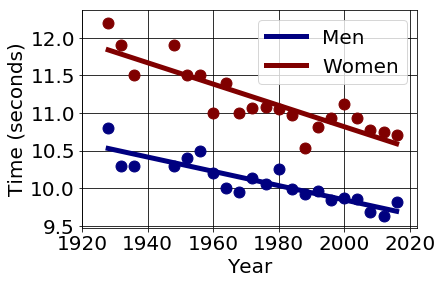
\includegraphics[width=0.4\textwidth]{img/chap1/sec1-3/fig1-3-dash-curve.png}\\
    \caption{Winning Olympic 100-Meter Dash Times with Models}
    \label{fig:1-3-dash-curve}
    \vspace{12pt}
\end{floatingfigure}
%\end{figure}
Note that we have all the necessary components of a model: (1) a description of the input variable ($y$), with the units (years), (2) a description of the functions ($m$ and $w$) and their units (seconds), and (3) a domain over which the models make sense. A plot of the models with the scatter plot of the data shows that the models make sense.

\begin{example}
Given the data in Table \ref{tab:1-3-dash} and the models in \eqref{eq:1-3-dash}, what are reasonable predictions for the winning times in the 100-meter dash at the 2020 Olympics?

\begin{solution}
Since $y$ is the year of the Olympics, then we predict the winning time for the men's 100-meter dash to be
$$m(2020) = -0.009498\cdot 2020 + 28.841\mbox{ seconds} = 9.66 \mbox{ seconds}$$
and for the women's 100-dash:
$$w(2020) = -0.014185\cdot 2020 + 39.188\mbox{ seconds} = 10.53 \mbox{ seconds.}$$

These times aren't completely unreasonable, given the data, but taken in context, one might be a bit skeptical of these predictions. For the men's 100-meter dash, the time of 9.66 would be only 0.03 slower than the Olympic record, held by Usain Bolt of Jamaica. Bolt ran the three fastest Olympic 100-meter dashes at the 2008, 2012, and 2016 Olympics, but has since retired from sprinting. The forecast women's time would beat Florence Griffith-Joyner's world record, set in 1988, by 0.01 second.
\end{solution}
\end{example}

To create a better model, we could include data from other races, not just the Olympics. We could also consider curves other than lines. To see why extrapolation has it's limitations with the linear model, consider the predicted winning times for the Olympics in the year 3000. For the men:
$$m(3000) = -0.009498\cdot 3000 + 28.841\mbox{ seconds} = 0.347 \mbox{ seconds}$$
and for the women's 100-meter dash:
$$w(3000) = -0.014185\cdot 3000 + 39.188\mbox{ seconds} = -3.37 \mbox{ seconds.}$$
These times are clearly absurd. The men's time would require a runner to run faster than a race car and for the women, no one can run a race in negative time. Therefore, the further out we attempt to extrapolate, the less plausible and more uncertain the results are.

The plot also gives us a question to consider. Notice that the women's times are decreasing more rapidly than the men's times. Will a woman ever run the 100 meter dash faster than a man in a single Olympics? The model predicts that this could happen, but the winning times would again be absurd.



% Curve-Fitting: testing/training.
